\section{Results and Conclusion}

\begin{frame}{Comparing Data Augmentations}
    \begin{itemize}
        \item WA is the most beneficial when robust overfitting is reduced.
    \item Spatial composition techniques which outperform blending techniques.
        \begin{figure}
            \centering
            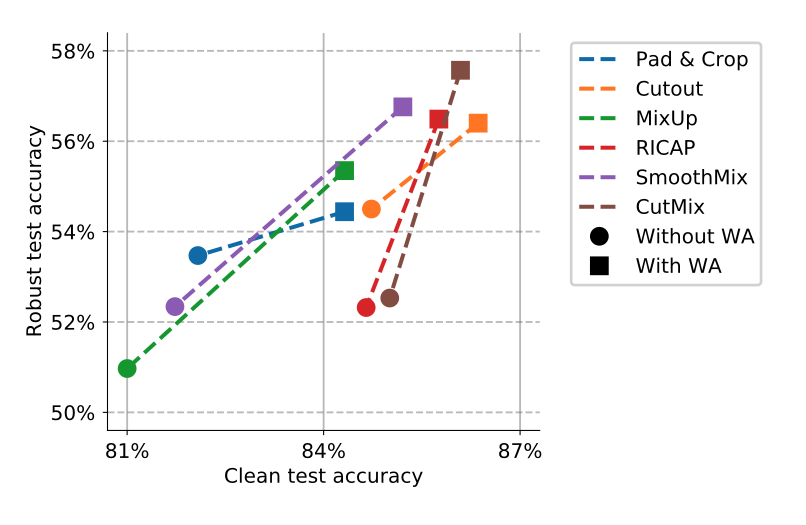
\includegraphics[height=.5\textheight]{pic/fig 4.png}
            \caption{Clean (without adversarial attacks) accuracy and robust accuracy (against AA+MT) for a WRN-28-10 trained against $\epsilon_\infty = 8/255$ on CIFAR-10 for different data augmentation techniques. The lines from circles to squares represent the performance change obtained when using WA.}
            \label{fig:fig4}
            \end{figure}
    \end{itemize}
\end{frame}

\begin{frame}{Blending Techniques}
    \begin{itemize}
        \item \textit{MixUp} samples the image mixing weight with a beta distribution $\text{Beta}(\alpha, \alpha)$
        \begin{itemize}
            \item tends to either produce images that are far from the original data distribution (when $\alpha$ is large)
            \item or too close to the original samples (when $\alpha$ is small)
        \end{itemize}
        \item Increasing $\alpha$ can lead to robust underfitting while an $\alpha$ too close to 0 would lead to robust overfitting.
        \begin{figure}
            \centering
            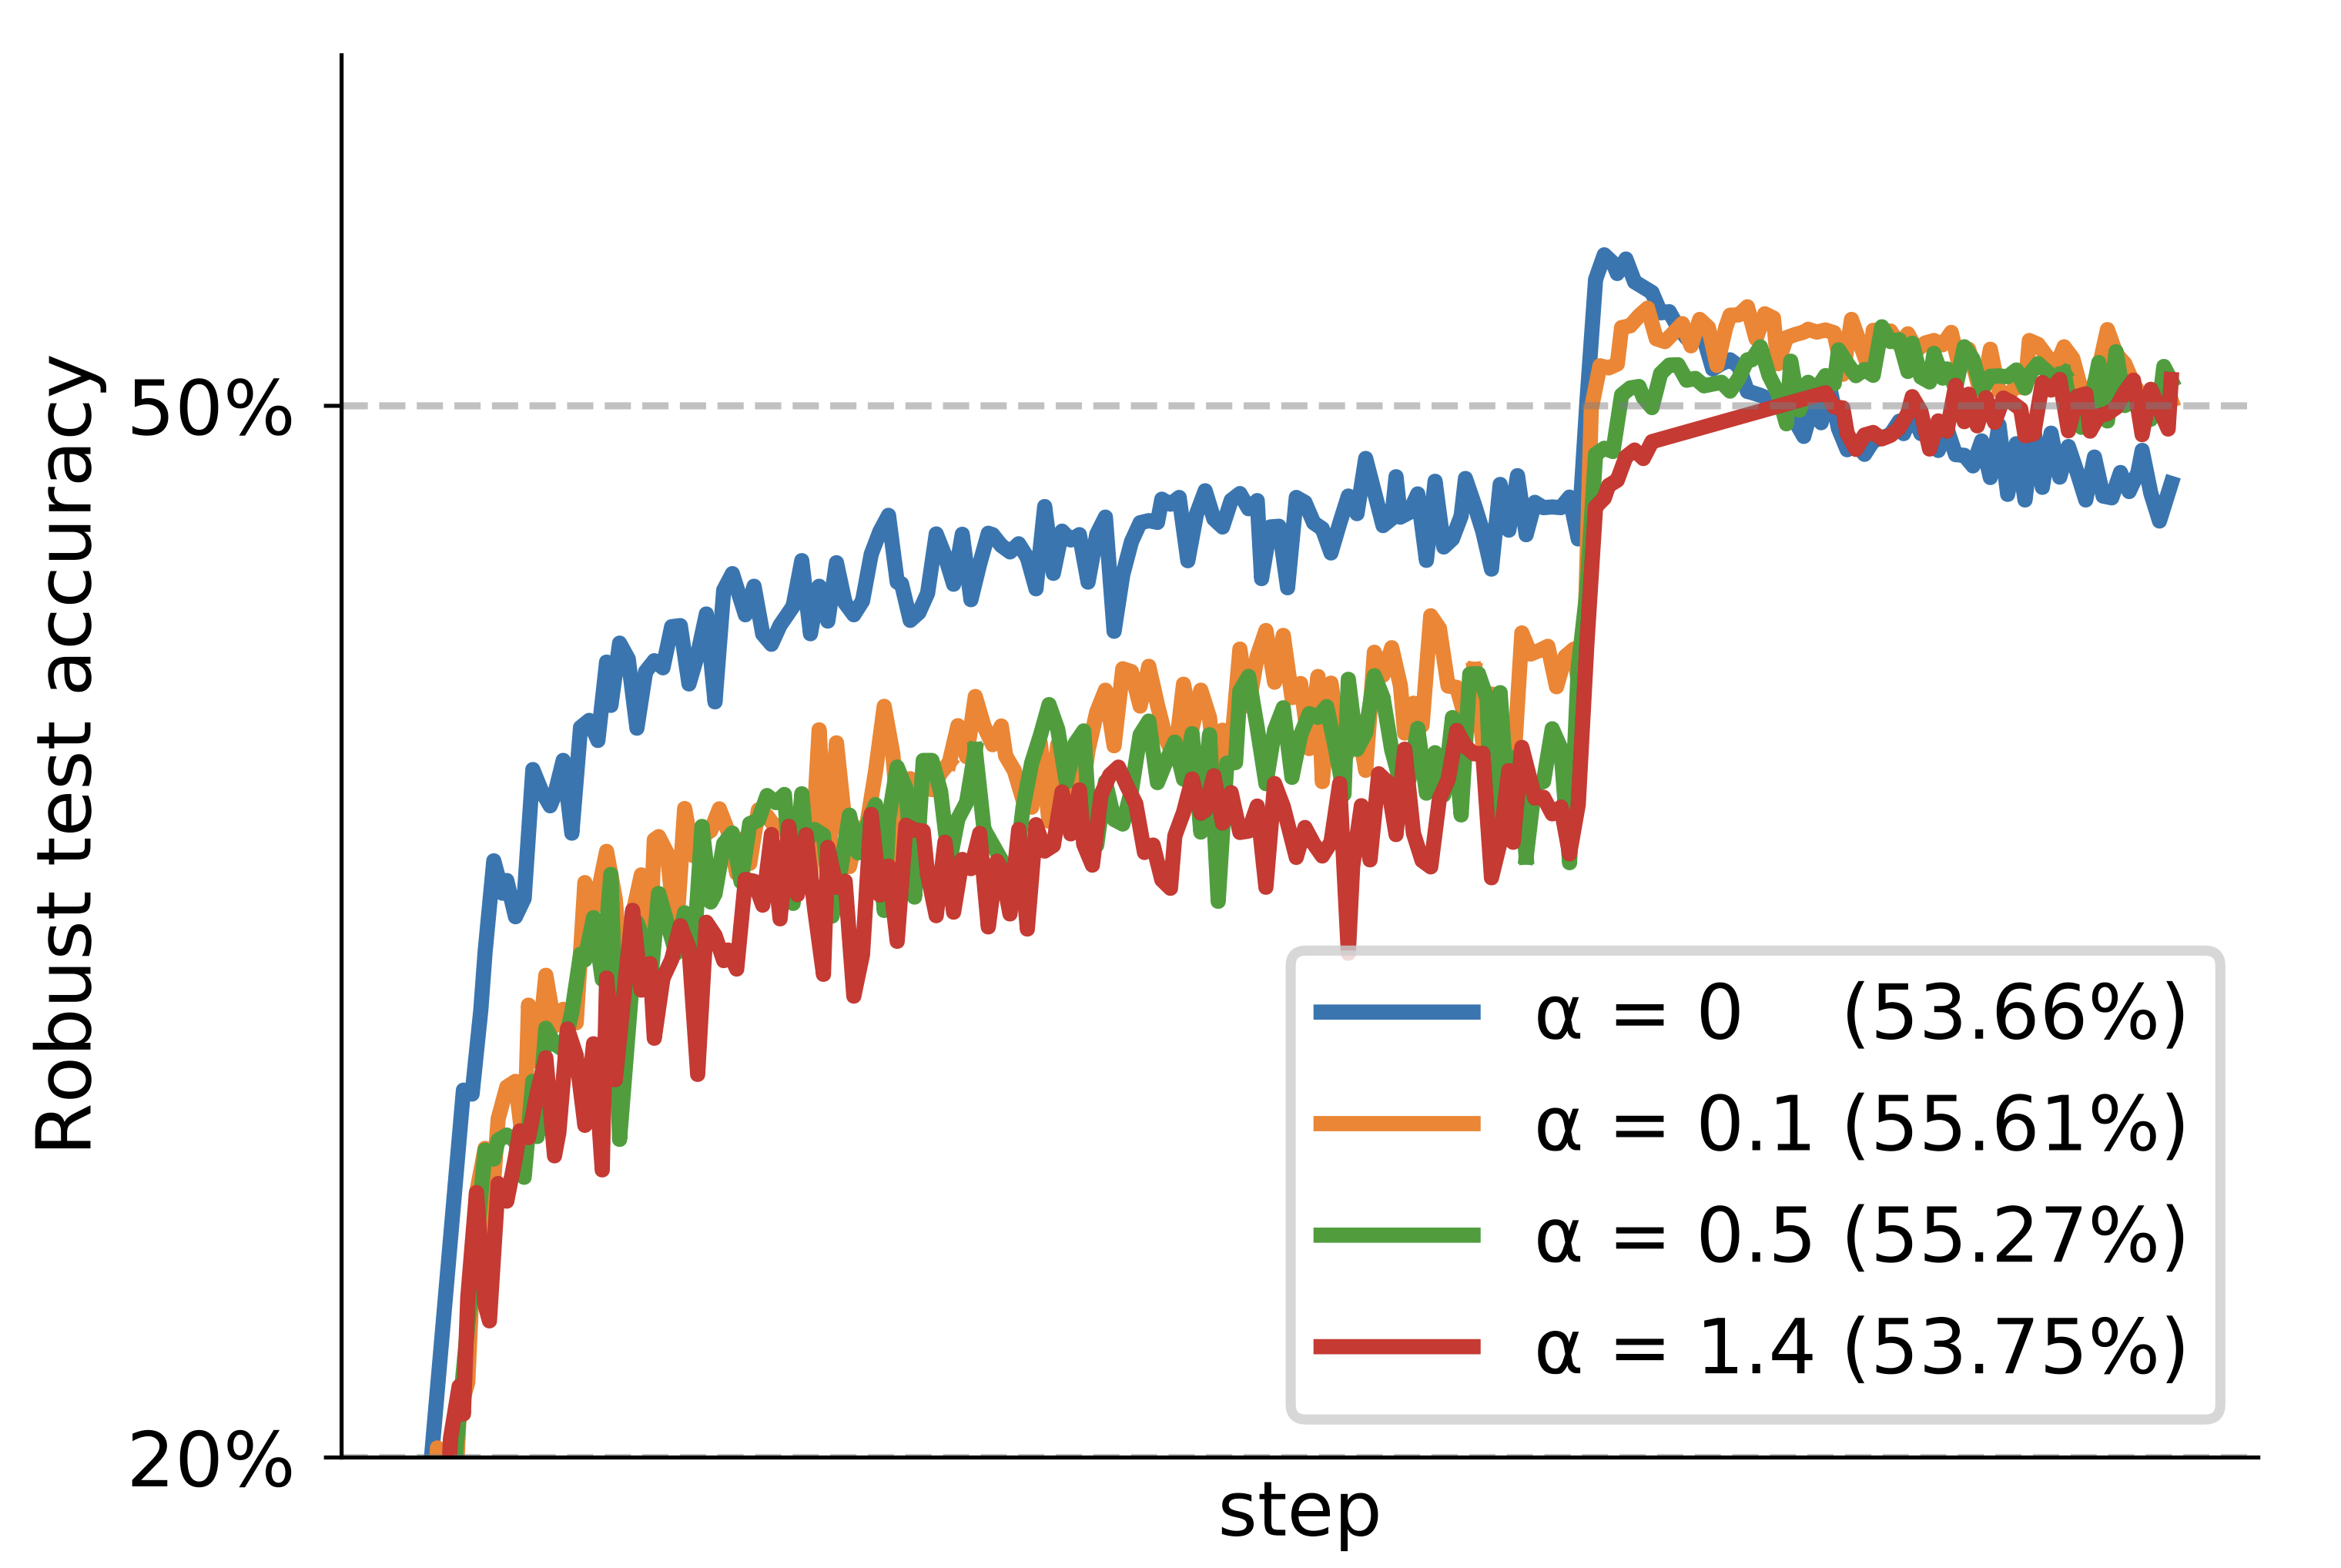
\includegraphics[height=0.4\textheight]{pic/mixup.png}
            \caption{The graph shows the robust test accuracy against $PGD^{40}$ with $\epsilon_\infty = 8/255$ on CIFAR-10 without using WA as we vary the mixing rate $\alpha$ of \textit{MixUp}. We report in the legend the robust accuracy (against AA+MT) after applying weight averaging to the corresponding runs.}
            \label{fig:fig5}
        \end{figure}
    \end{itemize}
\end{frame}

\begin{frame}{Spatial Composition Techniques}
\begin{itemize}
    \item \textit{Cutout} and \textit{CutMix} are most beneficial when using large window lengths.
    \item Low-level features tend to be destroyed by \textit{MixUp},
    \item whereas composition techniques locally maintain these low-level features. 
    \item Hence, we hypothesize augmentations designed for robustness need to preserve low-level features.
        \begin{figure}
            \centering
            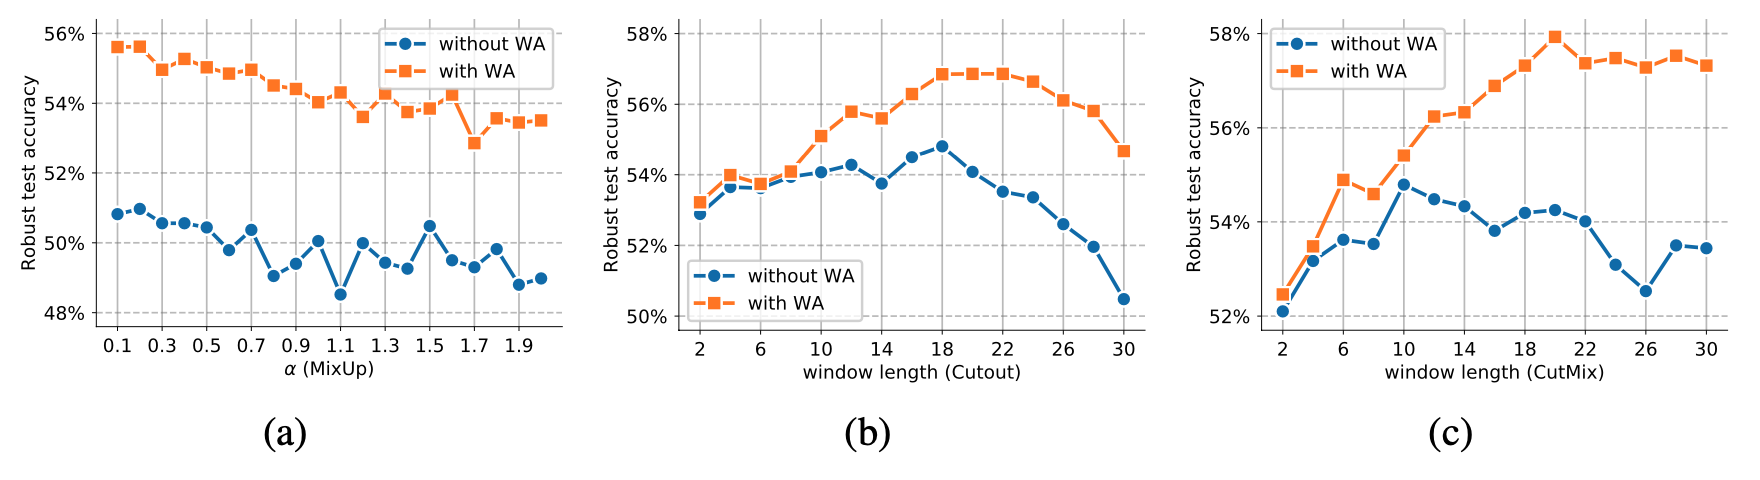
\includegraphics[height=.3\textheight]{pic/data_aug_res.png}
            \caption{Robust test accuracy against AA+MT with $\epsilon_\infty = 8/255$ on CIFAR-10 as we vary (a) the mixing rate α of MixUp, (b) the window length when using Cutout and (c) the window length when using CutMix. The model is a WRN-28-10 and we compare the settings without and with WA. 
            % As a reference when training only with Pad \& Crop, the same model with WA and without WA reaches $54.44\%$ and $53.66\%$ robust accuracy, respectively. Similarly, without any augmentation, the models with WA and without WA achieve $49.74\%$ and $42.27\%$, respectively.
            }
            \label{fig:data_aug_res}
        \end{figure}
    \end{itemize}
\end{frame}

\begin{frame}{Generalizing to other Architectures}
    \begin{figure}
        \centering
        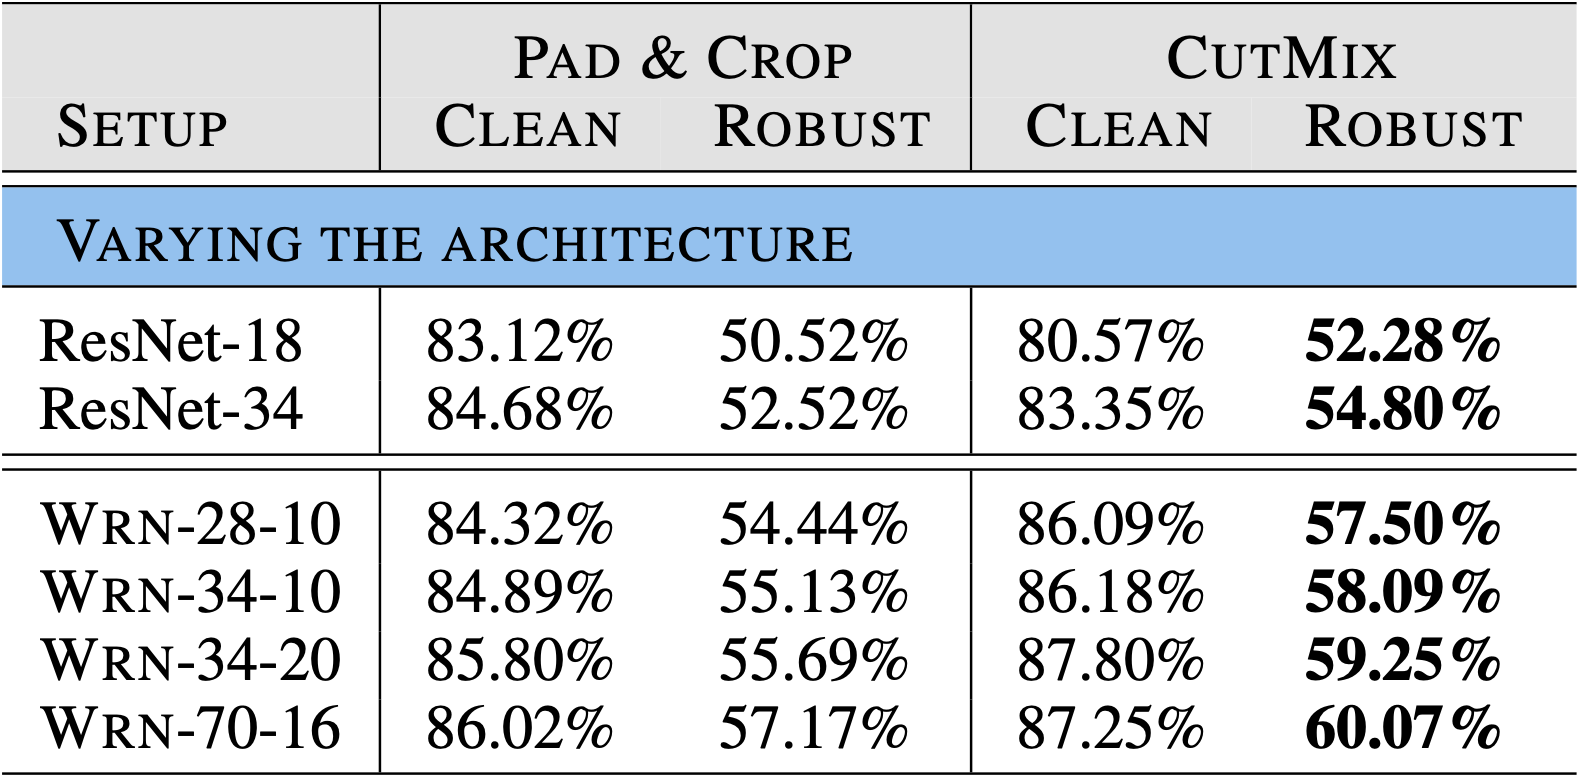
\includegraphics[width=\linewidth]{pic/Gen_Arch.png}
            \caption{Robust test accuracy (against AA+MT) against $\epsilon_\infty = 8/255$ on CIFAR-10 for different architectures. In all cases, we use weight averaging and we compare \textit{Pad \& Crop} and \textit{CutMix}.}
        \label{fig:gen_arch}
    \end{figure}
\end{frame}

\begin{frame}{Generalizing to other Threat Models}
    \begin{figure}
        \centering
            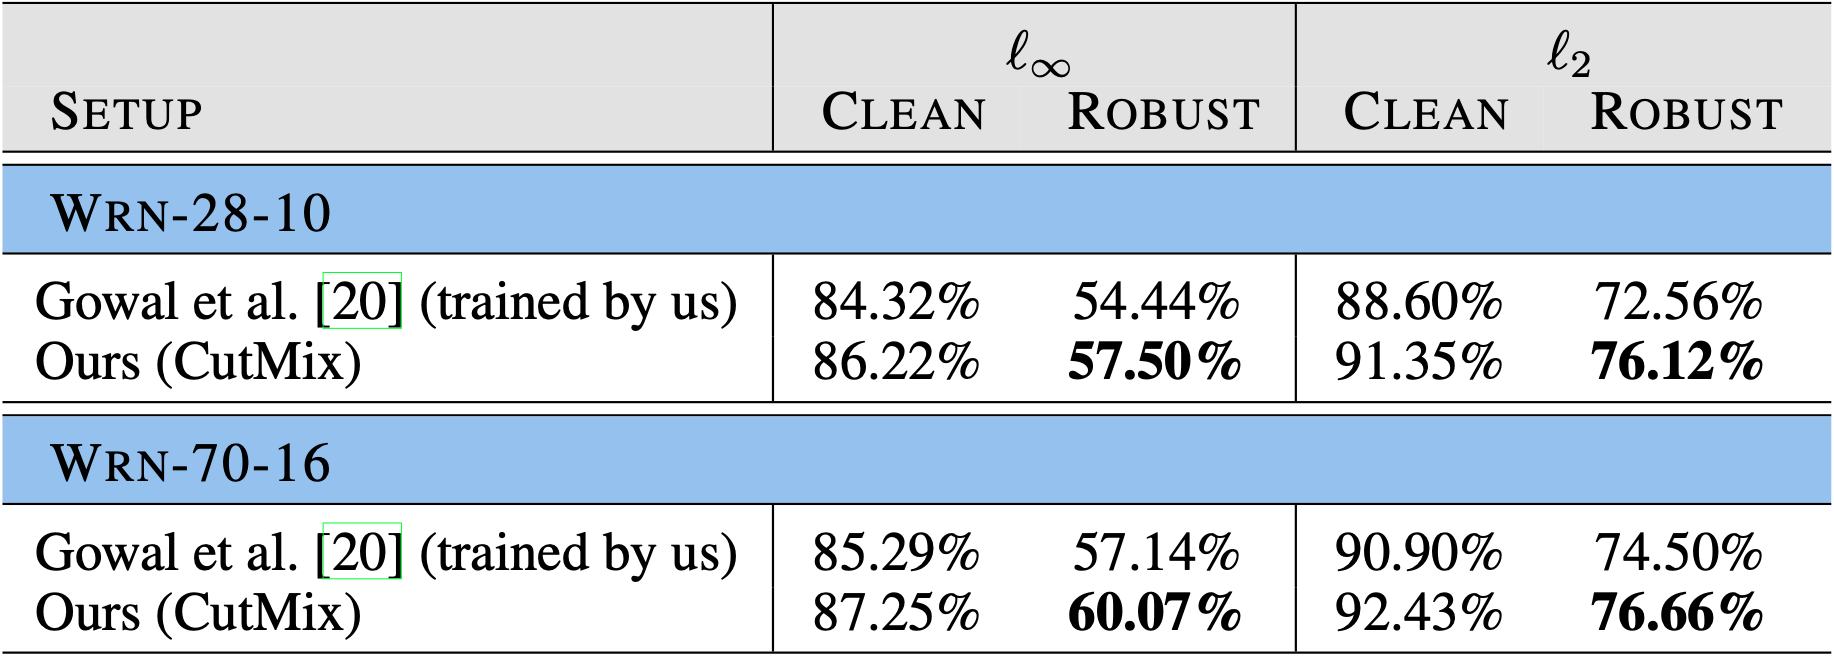
\includegraphics[width=\linewidth]{pic/Gen_Threat.png}
            \caption{Clean (with and without adversarial attacks) accuracy and robust accuracy (against AA+MT) on CIFAR-10 as we both test against $\epsilon_\infty = 8/255$ and $\epsilon_2 = 128/255$.}\label{fig:gen_threat}
    \end{figure}
\end{frame}

\begin{frame}{Generalizing to other Datasets}
    \begin{figure}
        \centering
        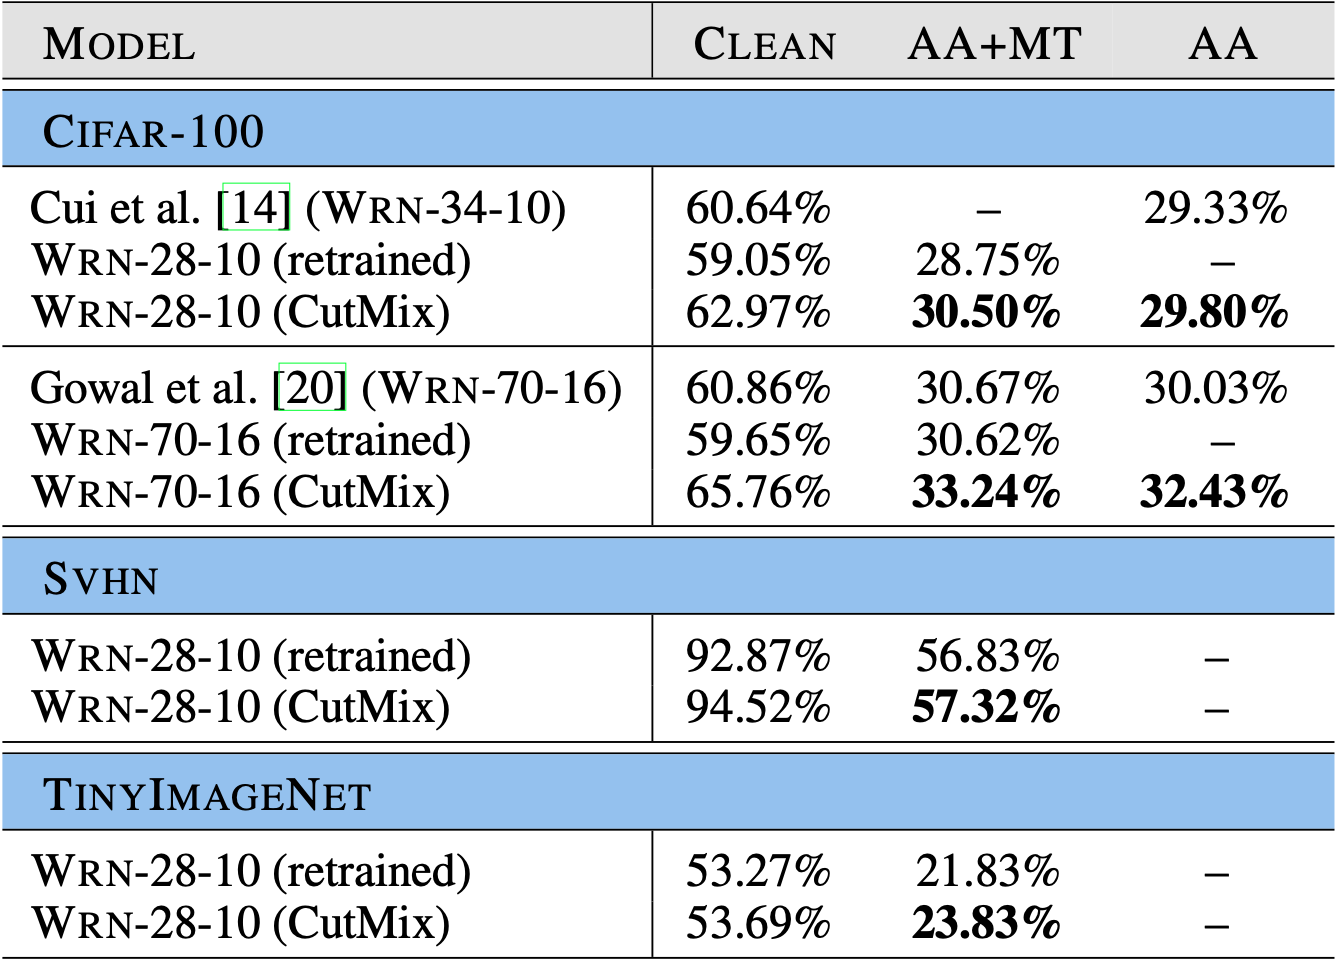
\includegraphics[width=0.7\linewidth]{pic/Gen_Data.png}
        \caption{Clean and robust accuracy (AA+MT and AutoAttack for select models) on CIFAR-100, SVHN and TINY-IMAGENET against $\epsilon_\infty = 8/255$ obtained by different models (with WA). The ’retrained’ indication means that the models have been retrained according to Gowal et al.’s methodology.}
        \label{fig:gen_data}
    \end{figure}
\end{frame}

\begin{frame}{Model Ensembling by Weight Averaging}
    Ensembling improves robustness by exploiting the diversity of equally performing models 
    \begin{figure}
        \centering
        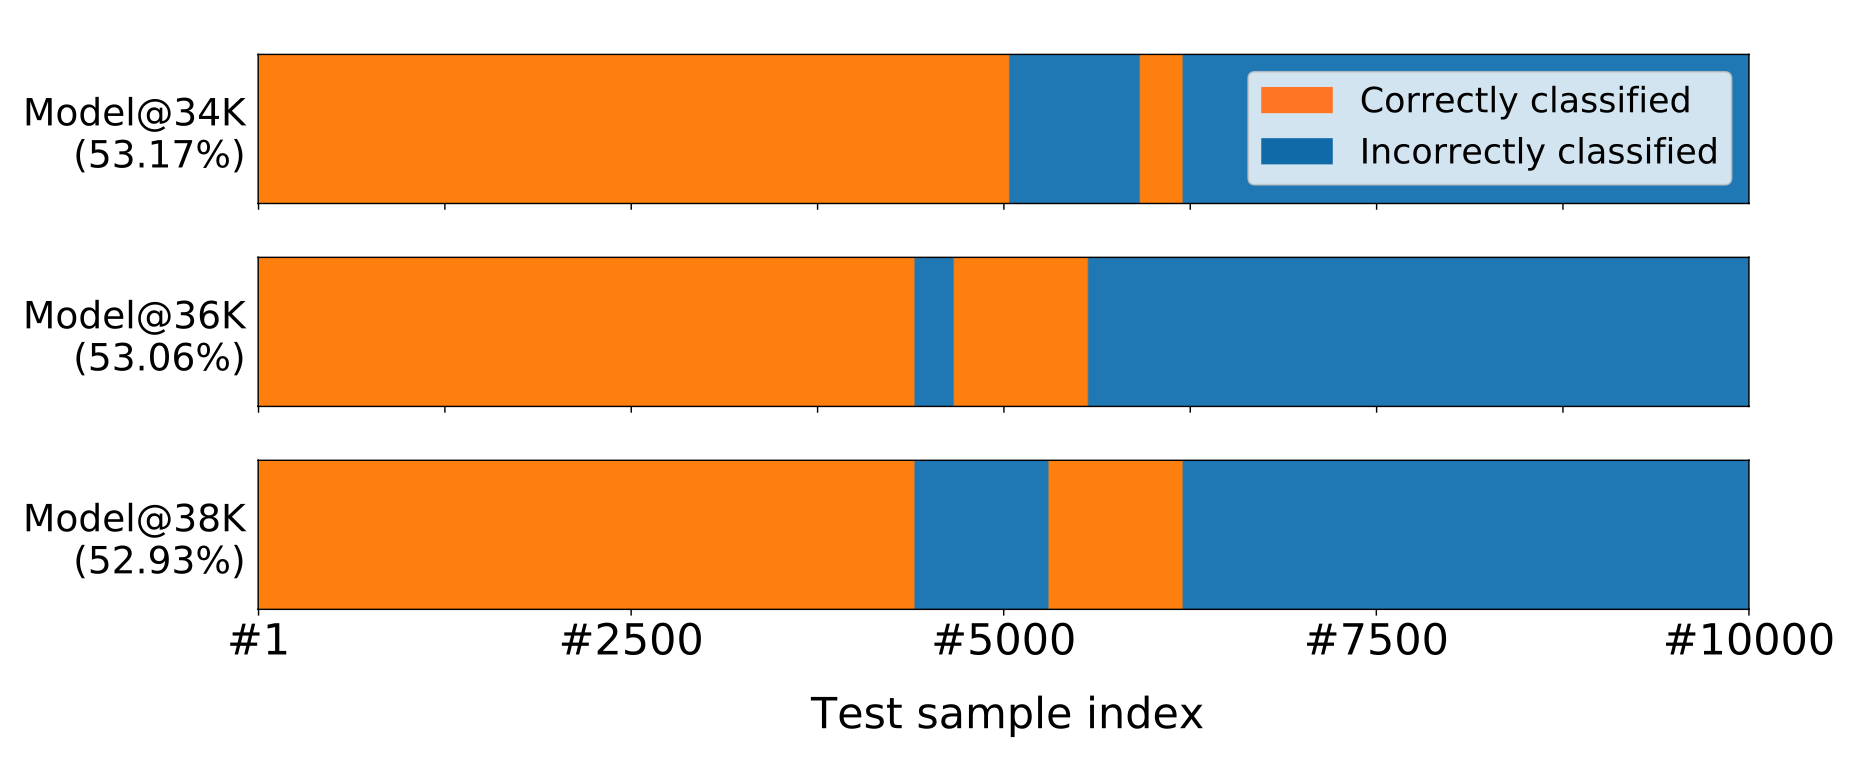
\includegraphics[width=\linewidth]{pic/fig 7.png}
        \caption{The bar plots show the outcome of each individual robust prediction for different snapshots of a same training run of a WRN-28-10 against $\epsilon_\infty = 8/255$ on CIFAR-10 without model weight averaging. The test sample indices have been re-ordered such as to show contiguous blocks. The plots show a significant variation in individual robust predictions across different snapshots while the total robust accuracy (i.e. the number in parenthesis) remains stable.}
        \label{fig:fig7}
    \end{figure}
\end{frame}

\begin{frame}{Limits of Exploiting Diversity}
The diversity between model iterations can only compensate up to a certain point for the decrease in robust performance due to robust overfitting.
    \begin{figure}
            \centering
            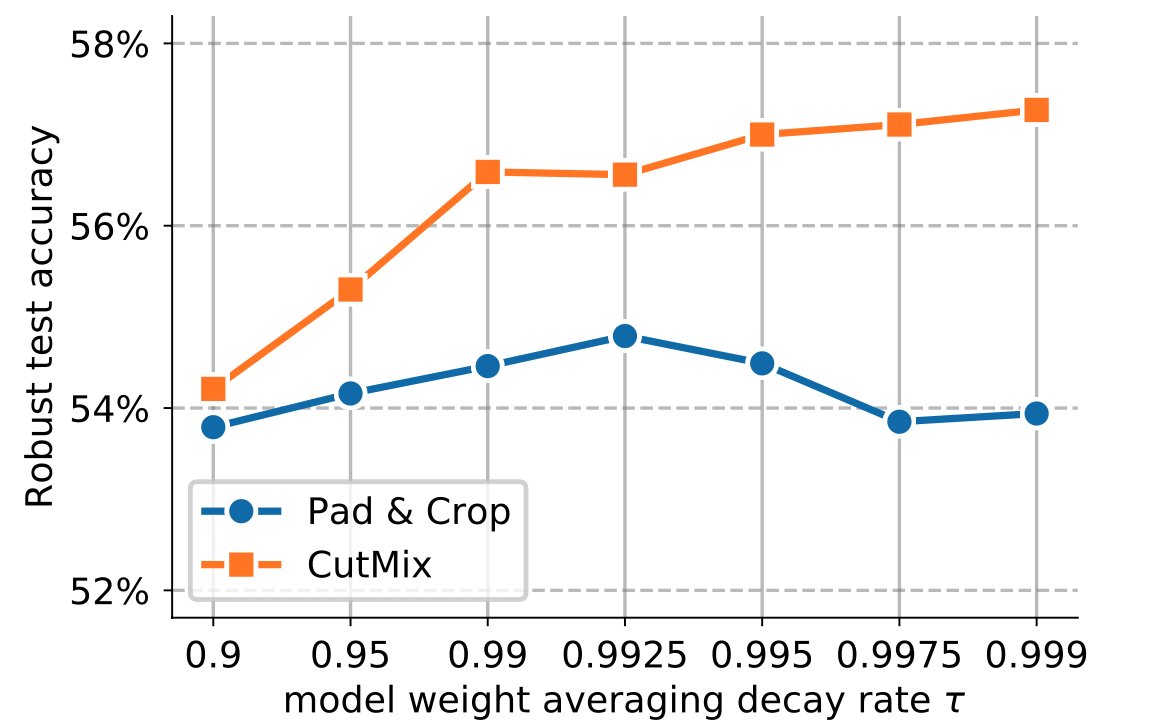
\includegraphics[width=0.7\linewidth]{pic/fig 8.png}
            \caption{Robust test accuracy against AA+MT with $\epsilon_\infty = 8/255$ on CIFAR-10 as we vary the decay rate of the model weight averaging. The model is a WRN-28-10, which is trained either with \textit{CutMix} or \textit{Pad \& Crop}.}
            \label{fig:fig8}
    \end{figure}
\end{frame}

\begin{frame}{Conclusion}
    \begin{itemize}[<+-| alert@+>] % stepwise alerts
        \item Contrary to previous works, which have tried data augmentation techniques to train adversarially robust models without success, we demonstrate that combining data augmentations with model weight averaging can significantly improve robustness.
        \item We also provide insights on why weight averaging works better with data augmentations which reduce robust overfitting.
        \item We show in fact that model snapshots of a same run have the same total robust accuracy but they greatly differ at the individual prediction level, thus allowing a performance boost when ensembling these snapshots.
    \end{itemize}
\end{frame}

\begin{frame}{Future Works}
    \begin{figure}
        \begin{minipage}{.45\textwidth}
            \centering
            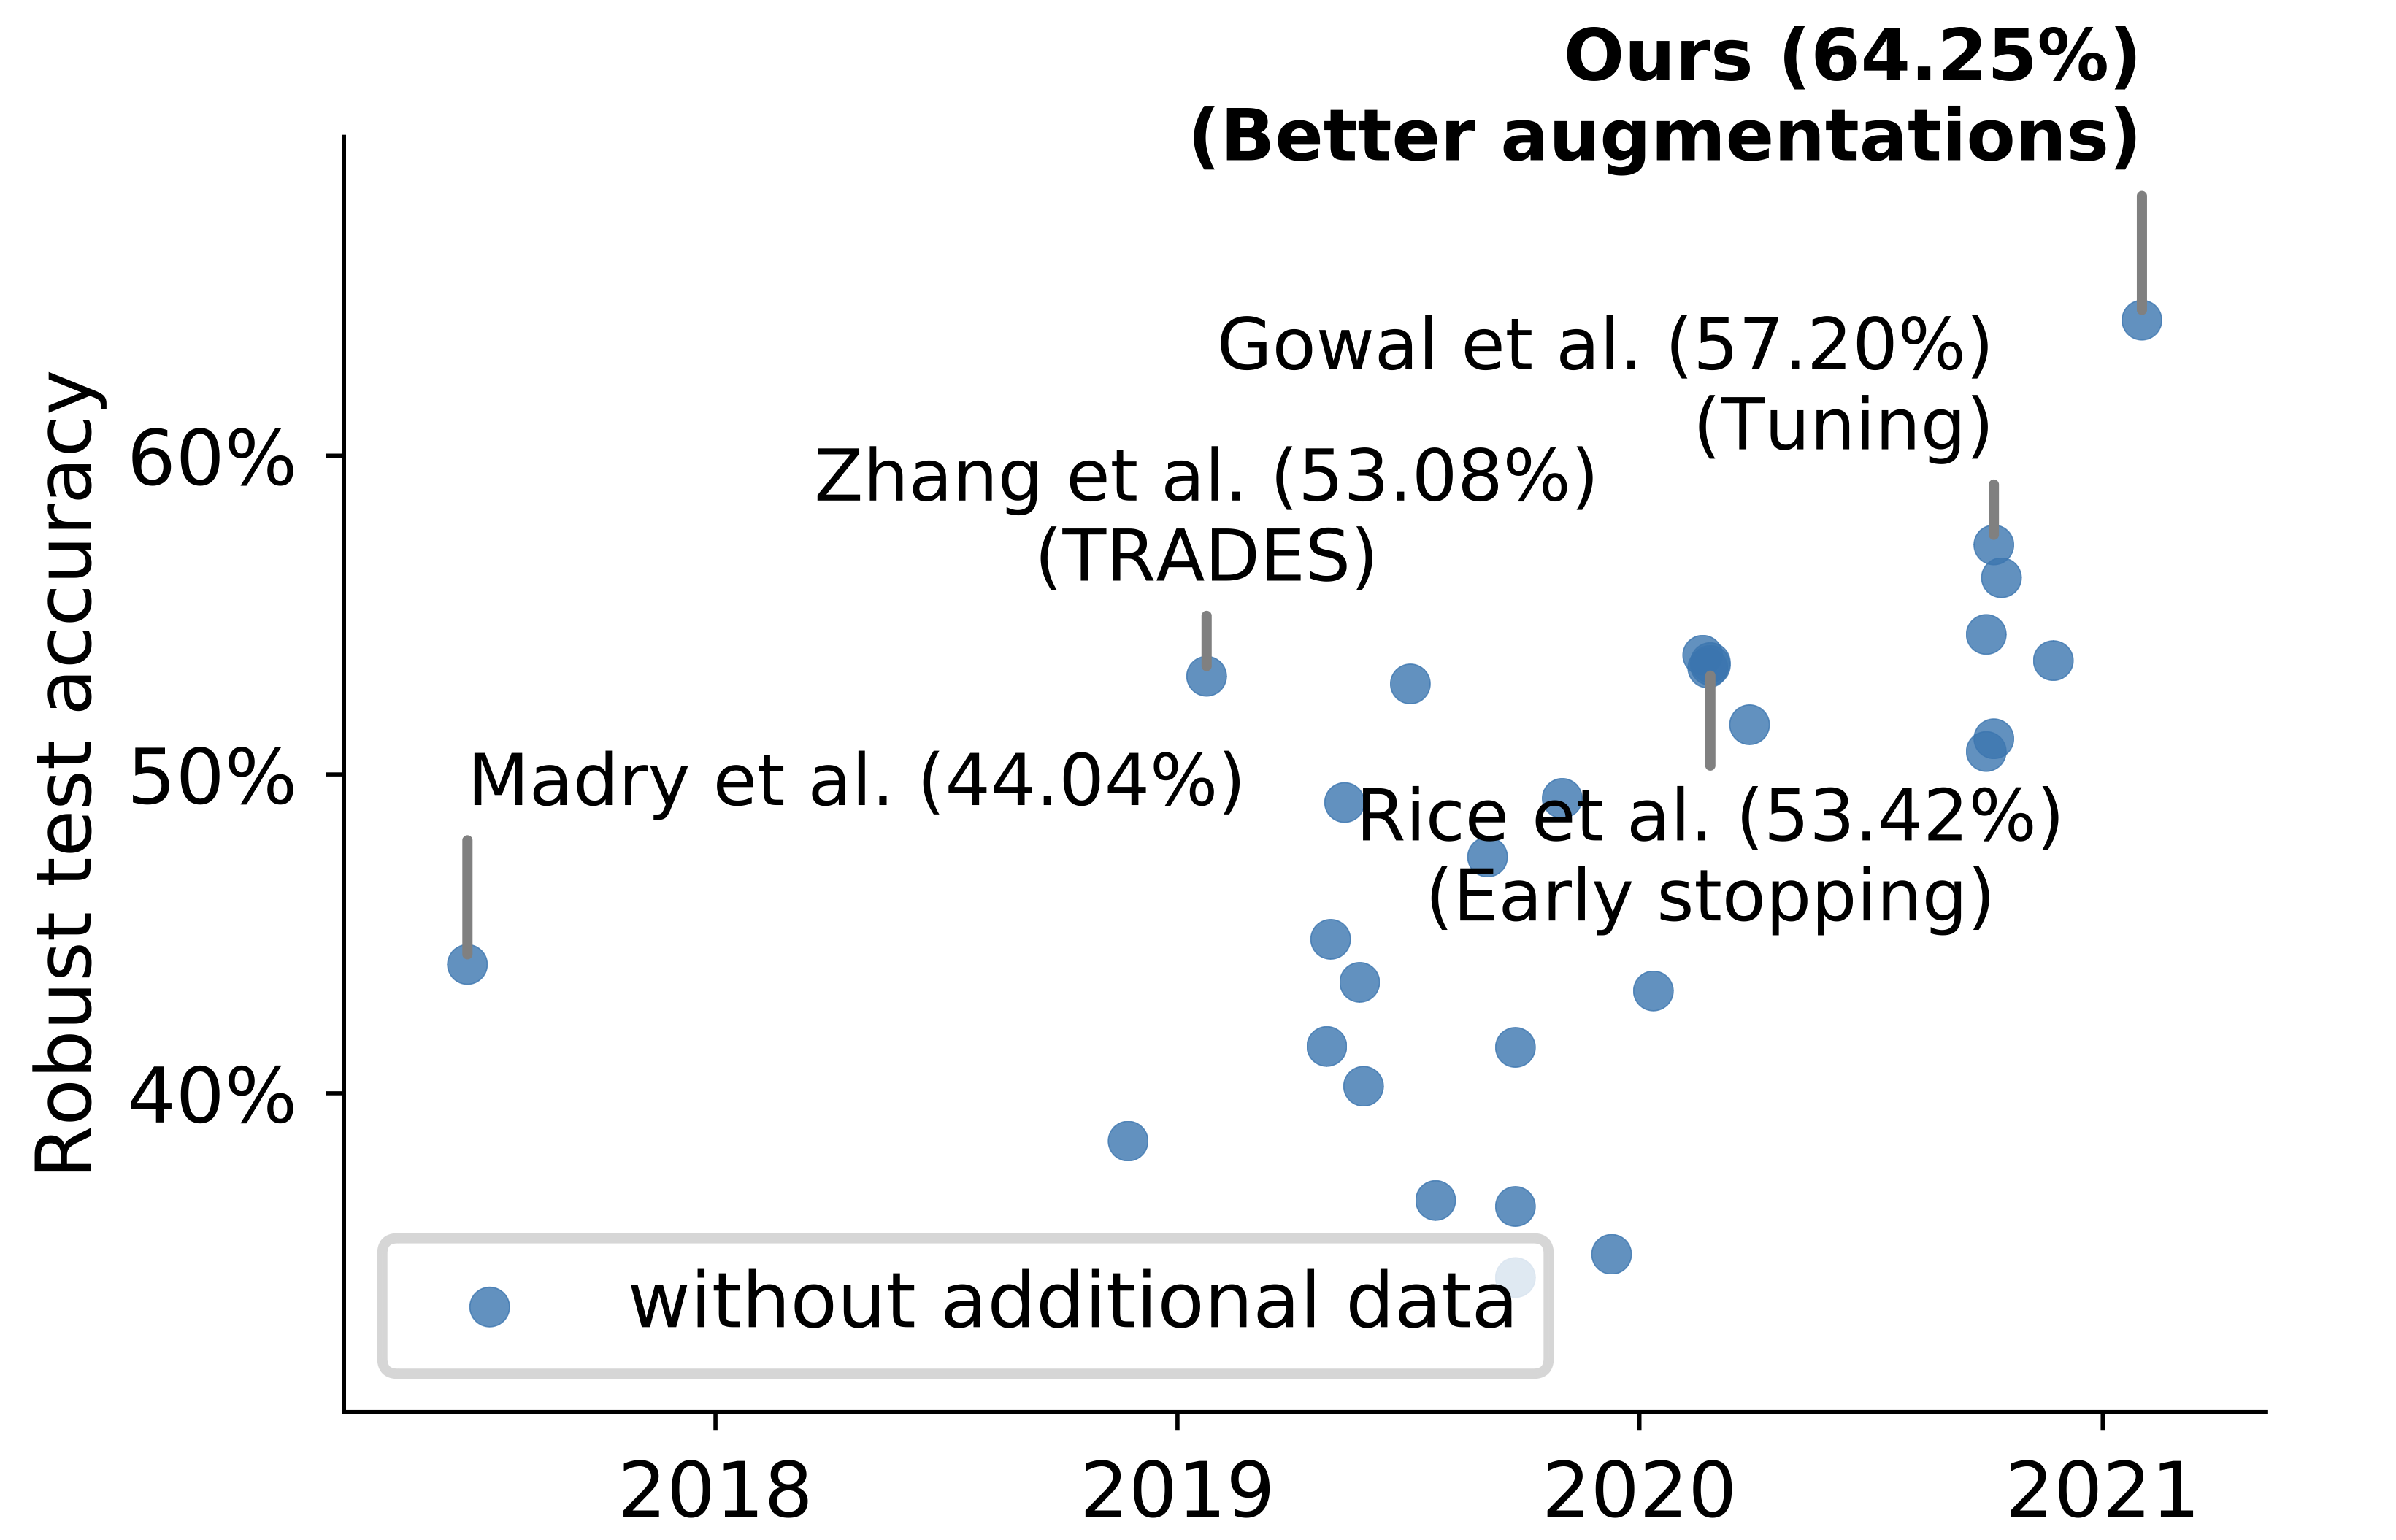
\includegraphics[width=\linewidth]{pic/oct 21.png}
            \caption{Fixing Data Augmentation to Improve Adversarial Robustness}
            \label{fig:oct21}
        \end{minipage}
        \begin{minipage}{.45\textwidth}
            \centering
            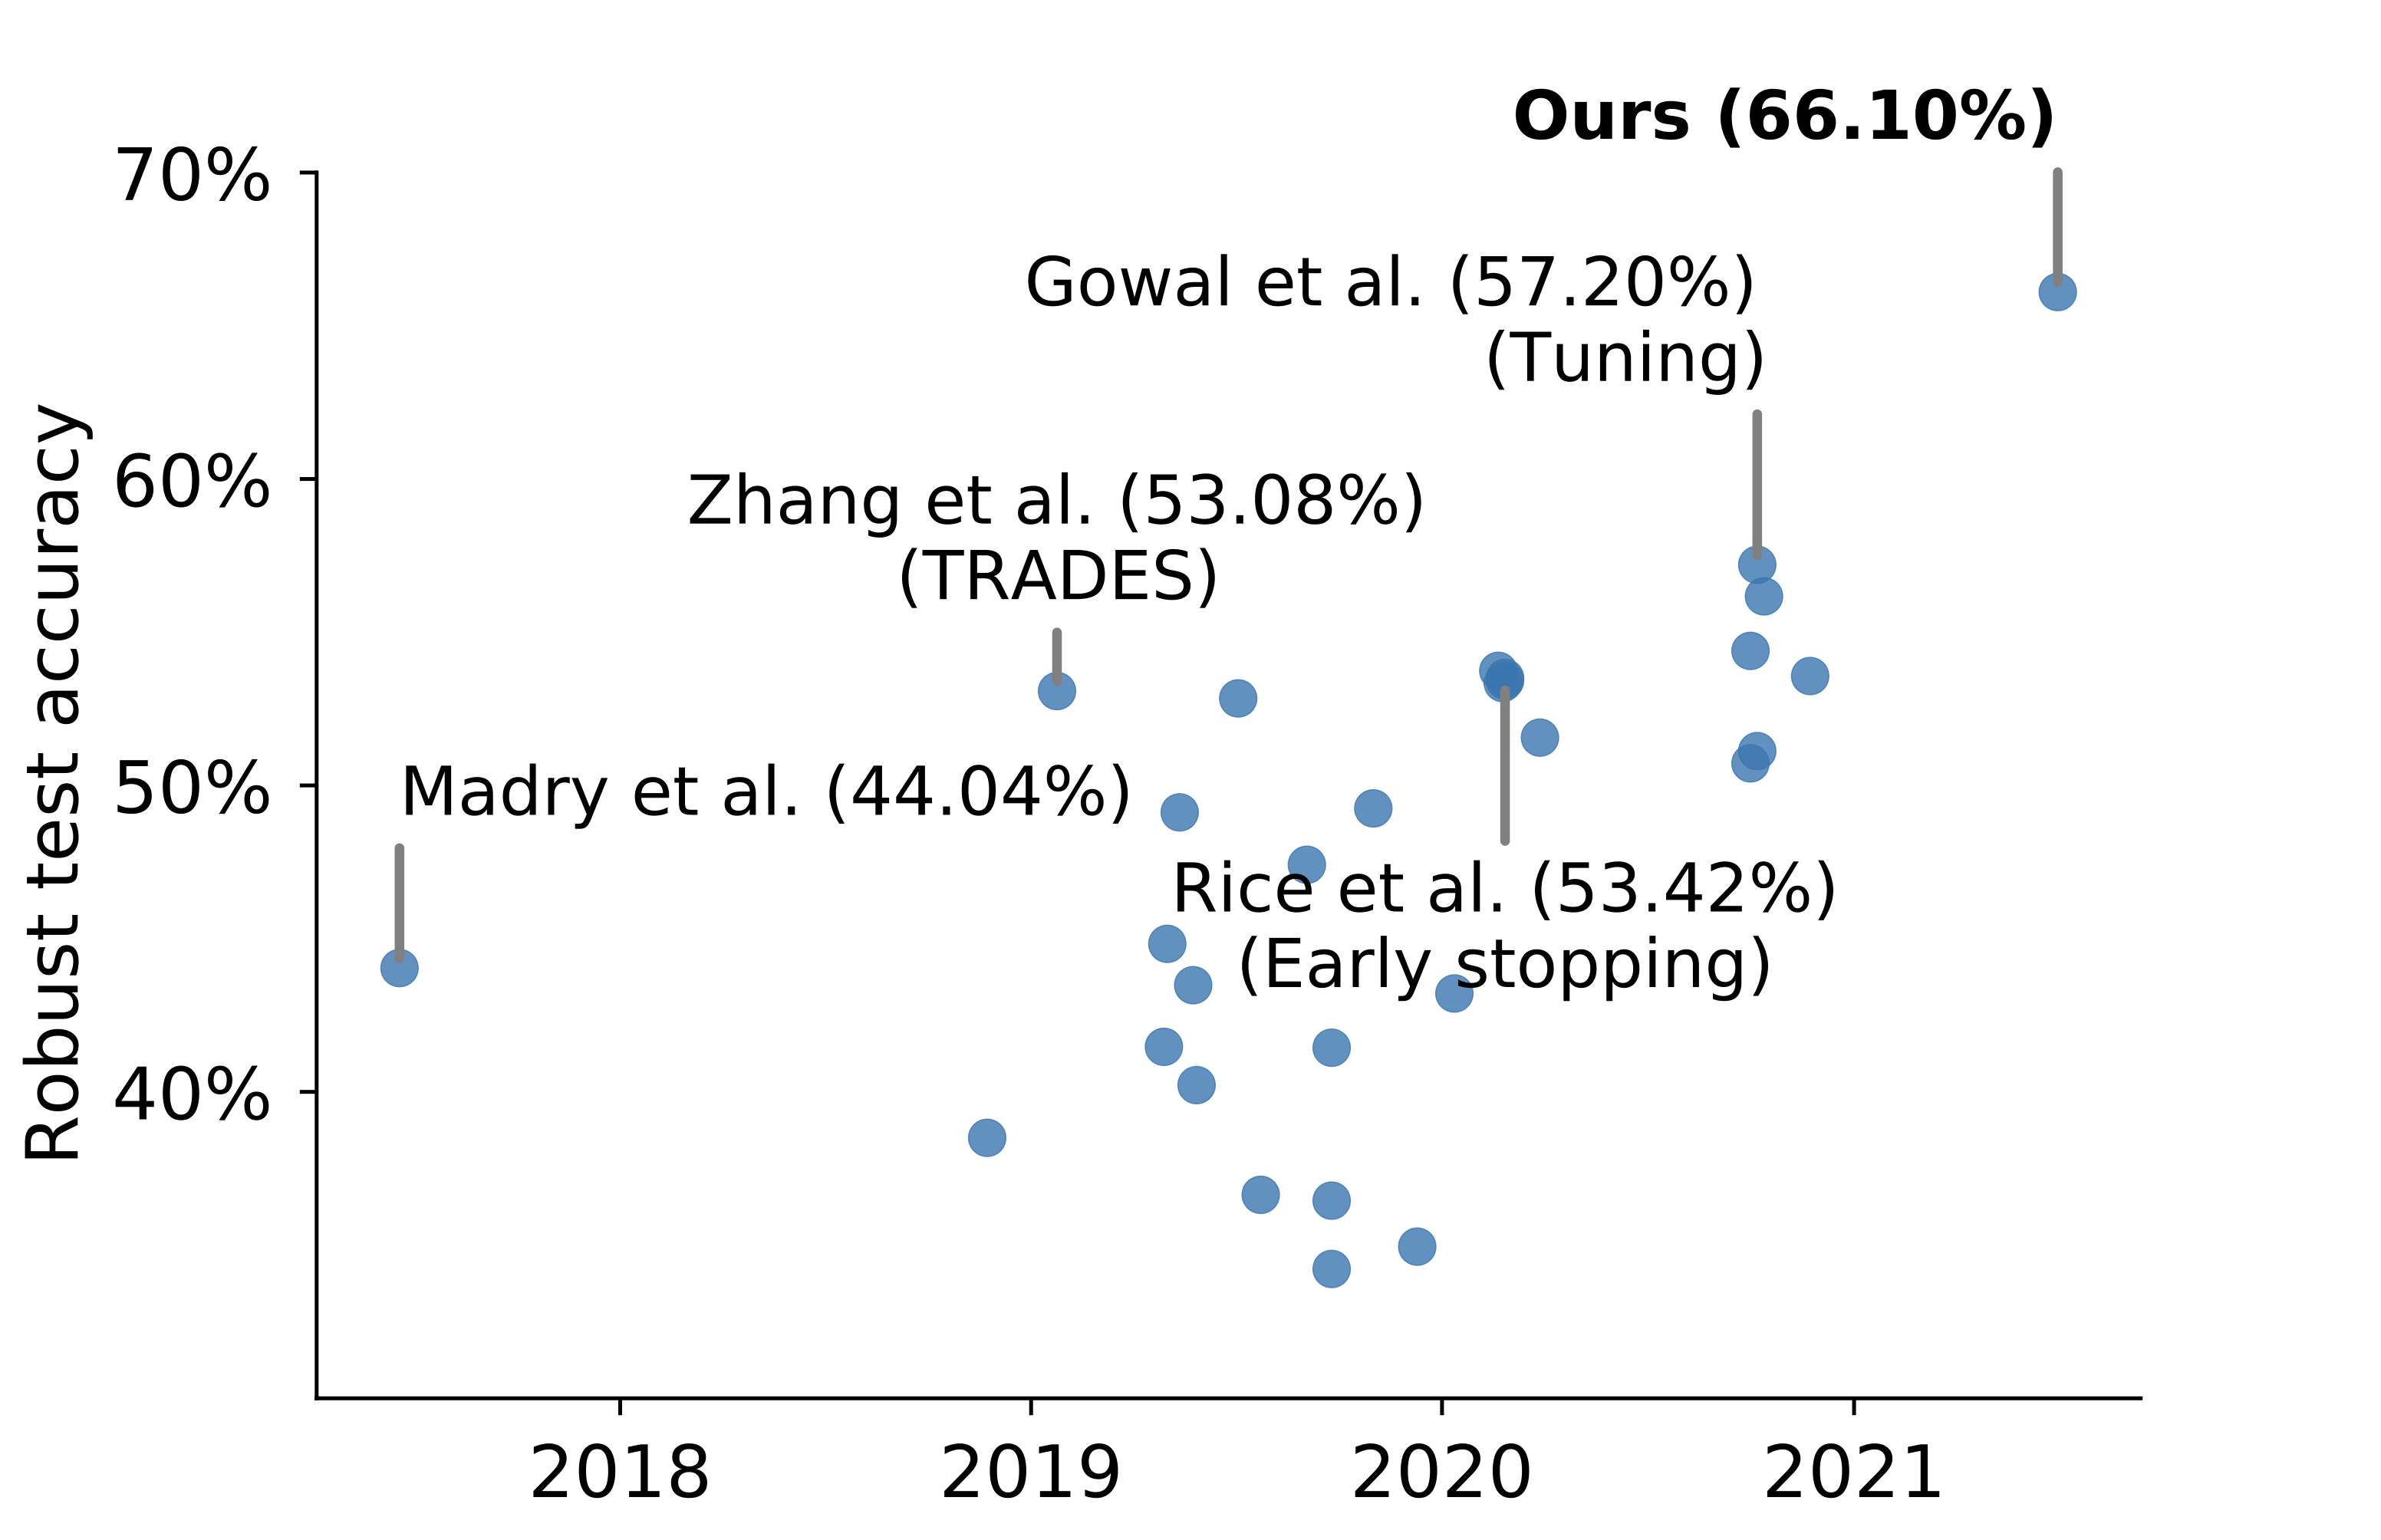
\includegraphics[width=\linewidth]{pic/dec 21.png}
            \caption{Improving Robustness using Generated Data}
            \label{fig:dec21}
        \end{minipage}
    \end{figure}
    
\end{frame}

\begin{frame}{Refrences}
    \bibliography{ref}
    \bibliographystyle{ieeetr}
    \nocite{*}
\end{frame}

% \begin{frame}
%     \begin{center}
%         {\Huge\calligra Thank You}
%     \end{center}
% \end{frame}